\documentclass[american]{scrartcl}

    \newcommand{\lang}{en}

    \usepackage{babel}
    \usepackage[utf8]{inputenc} 
    \usepackage{csquotes}
    \usepackage{amsmath, amssymb}
    \usepackage{graphicx}
    \usepackage{tikz} 
    \usepackage{mathtools}
    \usepackage{bm}

    \setlength{\parindent}{0em}
    \setlength{\parskip}{0.5em}
	\setlength{\fboxsep}{1em}


    % Graphs
    \usetikzlibrary{positioning, arrows.meta, calc, decorations.markings, math}

    \tikzset{main node/.style={circle, draw,minimum size=2cm,inner sep=3pt},}

    % Math commands
    \newcommand{\E}{\mathbb{E}}
    \newcommand{\R}{\mathbb{R}}

    \newcommand{\matr}[1]{\bm{#1}}
	\newcommand{\set}[1]{\left\{#1\right\}}

	\DeclareMathOperator{\Tr}{Tr}

    \DeclarePairedDelimiter\abs{\lvert}{\rvert}%
    \DeclarePairedDelimiter\norm{\lVert}{\rVert}%


    \usepackage[
        bibencoding=utf8, 
        style=apa
    ]{biblatex}

    \bibliography{../../../Desktop/bibliographies/thesis, ../maths}
    
    
    \usepackage{amsmath}
    \title{
        Prosumer Electricity Markets
    }

    \subtitle{Model}

    \author{Andrea Titton}
    
\begin{document}

\nocite{*}
\maketitle

\section{Network structure}

\begin{center}
	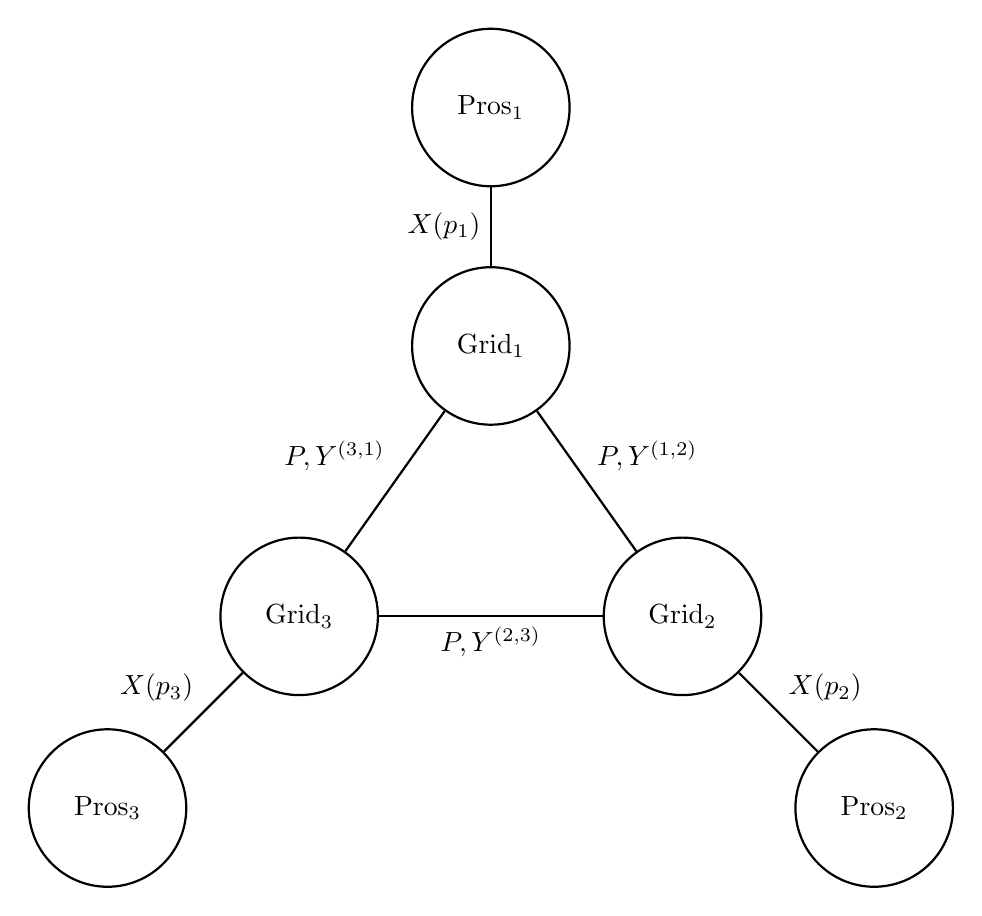
\begin{tikzpicture}[-, thick]
		% Grids
		\node[main node] (1) {Grid$_1$};
		\node[main node] [below right = 2cm and 1cm of 1] (2) {Grid$_2$};
		\node[main node] [below left = 2cm and 1cm of 1] (3) {Grid$_3$};
		% Local markets 
		\node[main node] [above = 1cm of 1] (5) {Pros$_1$};
		\node[main node] [below right = 1cm and 1cm of 2] (6) {Pros$_2$};
		\node[main node] [below left = 1cm and 1cm of 3] (7) {Pros$_3$};
		% Paths
		\path[draw,thick]
		(1) edge node [above right] {$P, Y^{(1, 2)}$} (2)
		(2) edge node [below] {$P, Y^{(2, 3)}$} (3)
		(3) edge node [above left] {$P, Y^{(3, 1)}$} (1)
		(1) edge node [left] {$X(p_{1})$} (5)
		(2) edge node [above right] {$X(p_{2})$} (6)
		(3) edge node [above left] {$X(p_{3})$} (7);
	\end{tikzpicture}
\end{center}

\section{Prosumers}

\subsection{Normal preferences}

The prosumer instantaneous utility of electricity consumption is,

\begin{equation*}
	u_i(x) = d_i \cdot \ln(x),
\end{equation*}

where $d_i$ is an heterogenous demand parameter.

Furthermore, agents get electricity endowment $e_{i, t}$ which follows a random exogenous process and have a given stock of cash-in-hand $m_t$, starting from $m_0$. Furthermore agents can buy or sell electricity $x_t$ at price $p_t$.

The dynamic optimization problem is then,

\begin{equation*}
	\begin{split}
		V(e_t) &= \sup_{x_t \in \R} \left\{u(x_t + e_t) + \beta \cdot \E_t V( e_{t+1} ) \right\} \\
		\\
		\textit{s.t. } m_{t+1} &= m_{t} - p_{t} \cdot x_{t}\\
		m_t  &\geq 0, \ m_0
	\end{split}
\end{equation*}

Hereafter we will suppress $i$ for convenience.

Agents are assumed to make forecasts over the price $p_{t+1}$, using a linear forecasting rule $\E_t[p_{t+1}] = \psi_h\cdot p_t$, where $\psi_h \in \Psi$ is selected in a manner similar to \citeauthor{Hommes2013} (\citeyear{Hommes2013}).

Using the budget constraint we can redefine the problem as,

\begin{equation}
	x_t = \frac{m_t - m_{t+1}}{p_t},
\end{equation}

such that the agents control variable is the next level of cash-in-hand $m_{t+1}$. This gives the Euler equation,

\begin{equation}
	u^\prime\left( e_t + \frac{m_t - m_{t+1}}{p_t} \right) = \beta \cdot \E_t \left[ u^\prime\left(e_{t+1} + \frac{m_{t+1} - m_{t+2}}{ \psi_h \cdot p_t} \right)  \right].
\end{equation}

The endogenous grid method can then be used to find a policy function

\begin{equation}
	m^\prime(m_t, p_t \ \vert \ \psi_h, e_t).
\end{equation}

The solution of the local problem yields the electricity demand in a state of high endowments and different conditions $m_t$ in Figure \ref{fig:demand} and the simulation run in Figure \ref{fig:sim}.

\begin{figure}[b]
	\centering
	\includegraphics[width=0.9\textwidth]{../../plots/markets/pricedemand.png}
	\label{fig:demand}
	\caption{Electricity demand curve for an agent}
\end{figure}

\begin{figure}
	\centering
	\includegraphics[width=0.9\textwidth]{../../plots/markets/simul.png}
	\label{fig:sim}
	\caption{Simulation of an agent with switching forecasting rule and $AR(1)$ price process}
\end{figure}

\begin{figure}
	\centering
	\includegraphics[width=0.9\textwidth]{../../plots/markets/kde.png}
	\label{fig:price}
	\caption{Prices in the above simulation}
\end{figure}

\iffalse
	\subsection{Epstein-Zin preferences}

	A better formulation, using Epstein-Zin preferences,

	\begin{equation}
		U_t = \left[ (1 - \beta) \cdot u(x_t)^{\frac{\phi - 1}{\phi}} + \beta \cdot \mu_t(U_{t+1})^{\frac{\phi - 1}{\phi}} \right]^{\frac{\phi}{\phi - 1}}
	\end{equation}

	where the certainty equivalent is,

	\begin{equation}
		\mu_t(U) = \E_t\left[ U^{1 - \gamma} \right]^{\frac{1}{1 - \gamma}}.
	\end{equation}

	As Caldara, introduce,

	\begin{equation}
		\theta := \frac{1 - \gamma}{1 - \frac{1}{\phi}}.
	\end{equation}

\fi

\section{Grid firms}

Grid firms face, each period, the optimization problem,

\begin{equation}
	\Pi_i\left(p_i, Y^{(i, j)}\right) = X_i(p_i) \cdot p_i - \sum_{j \in N(i)} Y^{(i, j)} \cdot P^{(i, j)},
\end{equation}
subject to,
\begin{equation}
	X_i=  \sum_{j \in N(i)} Y^{(i, j)}
\end{equation}

For now assume $P^{(i, j)}$ is determined by (i.e. is a function of) the vector of traded quantities $Y$, with elements $Y^{(l, m)} \ \forall \ l, m \in N$.

Suppressing $i$ for convenience (i.e. $Y^{(i, j)} \mapsto Y_j$), the Lagrangian is,

\begin{equation}
	\mathcal{L}\left(p, Y_j\right) = X(p) \cdot p - \sum_{j \in N(i)} Y_j \cdot P_j (Y) + \lambda\cdot \left(X(p) - \sum_{j \in N(i)} Y_j\right)
\end{equation}

with first order condition,

\begin{equation}
	\begin{split}
		\frac{\partial \mathcal{L}}{\partial p}  &= X^\prime(p) \cdot p + X(p) + \lambda \cdot X^\prime(p) = 0 \\
		\frac{\partial \mathcal{L}}{\partial Y^j}  &= P_j + \frac{\partial P_j}{\partial Y_j} \cdot Y_j + \lambda =0, \ \forall j \in N(i)
	\end{split}
\end{equation}

Isolating the multiplier $\lambda$ from the first equation yields,

\begin{equation}
	- \lambda = p + \frac{X}{X^\prime}(p)
\end{equation}

which yields the system of equations, $\forall j \in N(i)$,

\begin{equation} \label{firm_optimization}
	P_j(Y_j) + \frac{\partial P_j}{\partial Y_j} \cdot Y_j = p + \frac{X}{X^\prime}(p)
\end{equation}

\subsection{Bargaining model}

To solve the bargaining model we need to impose a ``direction'' of trade (i.e. $Y^{(i, j)} = - Y^{(j, i)}$). The grid network can then be thought of as a directed graph $\mathcal{A}$ with upper triangular adjacency matrix $\matr{A}_{d}$.

To encode the asymmetry of trade hereafter I will work with the bi-directred graph with adjacency matrix,

\begin{equation}
	\matr{A} := \matr{A}_{d} - \matr{A}_{d}^T,  \ \matr{A} \in\R^{n\times n}.
\end{equation}

This matrix has entries $a_{i, j} \in \set{-1, 0, 1}$ with $a_{i, j} = - a_{j, i}$ and $a_{i, i} = 0$. For example, the graph of Section 1 would then be represented by,

\begin{equation}
	\matr{A}_d= \begin{pmatrix}
		0 & 1 & 1 \\
		0 & 0 & 1 \\
		0 & 0 & 0
	\end{pmatrix} \implies
	\matr{A} = \begin{pmatrix}
		0 & 1 & 1 \\
		-1 & 0 & 1 \\
		-1 & -1 & 0
	\end{pmatrix}
\end{equation}

The payoff of firm $i \in N = \{1, \ldots, n\}$ from the bargaining procedure is then,

\begin{equation}
	\Pi_i\left( P^{(i, j)} \right) = X_i(p_i)\cdot p_i - \sum_{j \in N} a_{i, j} \cdot Y^{(i, j)} \cdot P^{(i, j)}.
\end{equation}

The Nash bargaining solution is such that,

\begin{equation}
	P^{(i, j)} = \arg \max_{P^{(i, j)}} \left\{\Pi_i \cdot \Pi_j \right\}.
\end{equation}

The first order condition is,

\begin{equation}
	\frac{\partial\Pi_i}{\partial P^{(i, j)}} \cdot \Pi_j + \frac{\partial\Pi_j}{\partial P^{(i, j)}} \cdot \Pi_i = 0.
\end{equation}

using,

\begin{equation}
	\frac{\partial\Pi_i}{\partial P^{(i, j)}} = - a_{i, j} \cdot Y^{(i, j)} = -\frac{\partial \Pi_j}{\partial P^{(i, j)}}
\end{equation}

we can rewrite the first order condition as,

\begin{equation} \label{foc_2}
	\begin{split}
		\Pi_i &= \Pi_j \\
		X_i(p_i)\cdot p_i - \sum_{m \in N} a_{i, m} \cdot Y^{(i, m)} \cdot P^{(i, m)} &= X_j(p_j)\cdot p_j - \sum_{m \in N} a_{j, m} \cdot Y^{(j, m)} \cdot P^{(j, m)}
	\end{split}
\end{equation}

Using $a_{i, j} = - a_{j, i}$, we can rewrite the two sums in (\ref{foc_2}) as,

\begin{equation}
	\begin{split}
		\sum_{m \in N} a_{i, m} \cdot Y^{(i, m)} \cdot P^{(i, m)} &= \sum_{m \in N \setminus \set{j}}  a_{i, m} \cdot Y^{(i, m)} \cdot P^{(i, m)} + a_{i, j} \cdot Y^{(i, j)} \cdot P^{(i, j)} \ \text{ and }\\
		\sum_{m \in N} a_{j, m} \cdot Y^{(j, m)} \cdot P^{(j, m)} &=  \sum_{m \in N \setminus \set{i}}  a_{j, m} \cdot Y^{(j, m)} \cdot P^{(j, m)} - a_{i, j} \cdot Y^{(i, j)} \cdot P^{(i, j)}
	\end{split}
\end{equation}

which yields, for every edge $(i, j)$ with $ a_{i, j} \neq 0$,

\begin{equation} \label{solution}
	\begin{split}
		P^{(i, j)} = \frac{1}{2\cdot Y^{(i, j)}} \Biggl( &\underbrace{X_i(p_i)\cdot p_i - X_j(p_j)\cdot p_j}_{\text{profit difference }}
		\\  + &\underbrace{\sum_{m\in N\setminus \set{i}} a_{j, m} \cdot Y^{(j, m)} \cdot P^{(j, m)}}_{\text{outside option of } j}
		\\ - & \underbrace{\sum_{m \in N\setminus \set{j}} a_{i, m} \cdot Y^{(i, m)} \cdot P^{(i, m)}}_{\text{outside option of } i} \Biggr).
	\end{split}
\end{equation}

\subsubsection{Line graph and matrix notation}

% FIXME: This is the incidence matrix

To write Equation (\ref{solution}) as a linear algebra problem I introduce the line graph associated with our original graph. In particular the line graph is the graph with adjacency matrix $\matr{L}(\matr{A}) \in \R^{\abs{E} \times \abs{E}}$ were nodes are edges of the original graphs and edges are inner nodes.

For example, consider the graph,

\fbox{
	\begin{minipage}{0.6\textwidth}
		\resizebox{\textwidth}{!}{
			\begin{tikzpicture}[{Latex[scale=1.25]}-{Latex[scale=1.25]}, thick]
				% Grids
				\node[main node] (1) {$1$};
				\node[main node] [right = 2cm of 1] (2) {$2$};
				\node[main node] [below right = 2cm and 2cm of 2] (5) {$5$};
				\node[main node] [above right = 2cm and 2cm of 2] (3) {$3$};
				\node[main node] [right = 2cm of 3] (4) {$4$};
				% Paths
				\path[draw,thick]
				(1) edge node [above] {$(1, 2)$} (2)
				(2) edge node [below left] {$(2, 5)$} (5)
				(2) edge node [above left] {$(2, 3)$} (3)
				(3) edge node [above] {$(3, 4)$} (4);
			\end{tikzpicture}}
	\end{minipage} \hfill
	\begin{minipage}{0.35\textwidth}
		\begin{equation*}
			\matr{A} = \begin{pmatrix}
				0  & 1  & 0  & 0 & 0 \\
				-1 & 0  & 1  & 0 & 1 \\
				0  & -1 & 0  & 1 & 0 \\
				0  & 0  & -1 & 0 & 0 \\
				0  & -1 & 0  & 0 & 0
			\end{pmatrix}
		\end{equation*}
	\end{minipage}
}

The corresponding line graph is,

\fbox{
	\begin{minipage}{0.6\textwidth}
		\resizebox{\textwidth}{!}{
			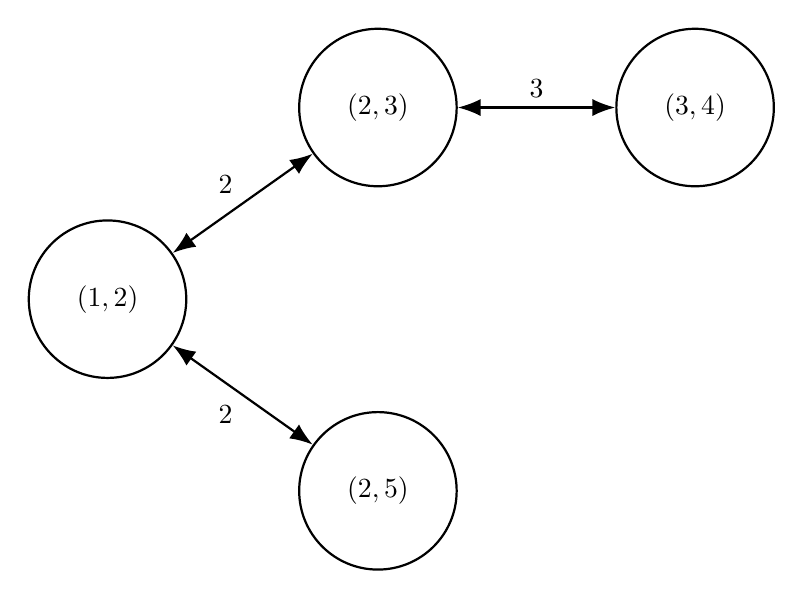
\begin{tikzpicture}[{Latex[scale=1.25]}-{Latex[scale=1.25]}, thick]
				% Grids
				\node[main node] (12) {$(1, 2)$};
				\node[main node] [below right = 1cm and 2cm of 12] (25) {$(2, 5)$};
				\node[main node] [above right = 1cm and 2cm of 12] (23) {$(2, 3)$};
				\node[main node] [right = 2cm of 23] (34) {$(3, 4)$};
				% Paths
				\path[draw,thick]
				(12) edge node [below left] {$2$} (25)
				(12) edge node [above left] {$2$} (23)
				(23) edge node [above] {$3$} (34);
			\end{tikzpicture}}
	\end{minipage} \hfill
	\begin{minipage}{0.35\textwidth}
		\begin{equation*}
			\matr{G}(\matr{A}) = \begin{pmatrix}
				0   & 1 & 1   & 0 \\
				- 1 & 0 & 0   & 0 \\
				- 1 & 0 & 0   & 1 \\
				0   & 0 & - 1 & 0
			\end{pmatrix}
		\end{equation*}
	\end{minipage}
}



\subsubsection{Line graph and bargaining solution}

In the bargaining problem we have a set of directed edges $E = \set{(i, j): i, j \in N}$. On each each a bargaining price and a transferred quantity is determined. This defined the two vectors $P, \ Y \in \R^{\abs{E}}$. Furthermore let $\Delta X$ in $\R^{\abs{E}}$ be the vector of profit difference with entries,

\begin{equation}
	\Delta X^{(i, j)} = X_i(p_i) \cdot p_i - X_{j}(p_j) \cdot p_j
\end{equation}

Equation (\ref{solution}) can be then written as,

\begin{equation} \label{matrix_solution}
	\begin{split}
		2(P \circ Y) &= \Delta X - \matr{G} \left( P \circ Y \right) \\
		(2\matr{I} + \matr{G}) (P \circ Y) &= \Delta X \\
		(P \circ Y) &= (2\matr{I} + \matr{G})^{-1} \Delta X \\
		P &= (2\matr{I} + \matr{G})^{-1} (\Delta X \oslash Y)
	\end{split}
\end{equation}

where $\circ$ and $\oslash$ denote the element-wise (Hadamard) product and division respectively.

\subsection{Solution of the bargaining problem}

Note that (\ref{matrix_solution}) defines the bargaining price as a function of the traded quantity $P(Y)$.

We can use this in equation (\ref{firm_optimization}),

\newpage

\section{Toy example with three firms}

Assume there are three grid firms, \hspace{2em}

\vspace{0.5cm}
\begin{minipage}{0.6\textwidth}
	\resizebox{\textwidth}{!}{
		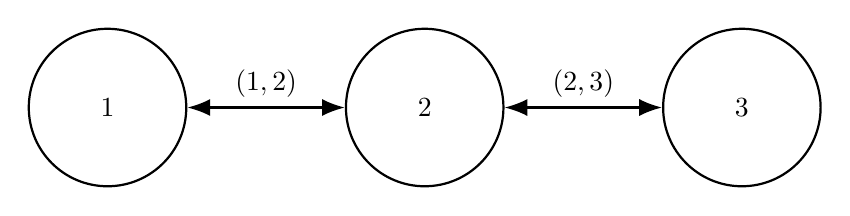
\begin{tikzpicture}[{Latex[scale=1.25]}-{Latex[scale=1.25]}, thick]
			% Grids
			\node[main node] (1) {$1$};
			\node[main node] [right = 2cm of 1] (2) {$2$};
			\node[main node] [right = 2cm of 2] (3) {$3$};
			% Paths
			\path[draw,thick]
			(1) edge node [above] {$(1, 2)$} (2)
			(2) edge node [above] {$(2, 3)$} (3);
		\end{tikzpicture}
	}
\end{minipage} \hfill
\begin{minipage}{0.35\textwidth}
	\begin{equation*}
		\matr{A} = \begin{pmatrix}
			0   & 1  & 0 \\
			- 1 & 0  & 1 \\
			0   & -1 & 0
		\end{pmatrix}
	\end{equation*}
\end{minipage}
\vspace{0.5cm}


and the associated line graph is,

\vspace{0.5cm}
\begin{minipage}{0.6\textwidth}
	\resizebox{0.7\textwidth}{!}{
		\begin{tikzpicture}[{Latex[scale=1.25]}-{Latex[scale=1.25]}, thick]
			% Grids
			\node[main node] (12) {$(1, 2)$};
			\node[main node] [right = 2cm of 1] (23) {$(2, 3)$};
			% Paths
			\path[draw,thick]
			(12) edge node [above] {$2$} (23);
		\end{tikzpicture}
	}
\end{minipage} \hfill
\begin{minipage}{0.35\textwidth}
	\begin{equation*}
		\matr{G} = \begin{pmatrix}
			0  & 1 \\
			-1 & 0
		\end{pmatrix}
	\end{equation*}
\end{minipage}
\vspace{0.5cm}



The Nash bargaining solution is then

\begin{equation*}
	\begin{split}
		\begin{pmatrix}
			P^{(1, 2)} \cdot Y^{(1, 2)} \\
			P^{(2, 3)} \cdot Y^{(2, 3)}
		\end{pmatrix} &= (2\matr{I} + \matr{G})^{-1} \Delta X \\
		&= \begin{pmatrix}
			2  & 1 \\
			-1 & 2
		\end{pmatrix}^{-1} \Delta X = \begin{pmatrix}
			0.4 & -0.2 \\
			0.2 & 0.4
		\end{pmatrix} \Delta X \\
		\implies P &= \begin{pmatrix}
			0.4 & -0.2 \\
			0.2 & 0.4
		\end{pmatrix} (\Delta X \oslash Y)
	\end{split}
\end{equation*}

Denoting with $\partial P$ the vector of partial derivatives $\frac{\partial P^{i, j}}{\partial Y^{i, j}}$ (diagonal of the Jacobian), we can write,

\begin{equation}
	\begin{split}
		P + \partial P \circ Y &= \begin{pmatrix}
			0.4 & -0.2 \\
			0.2 & 0.4
		\end{pmatrix} (\Delta X \oslash Y) - 0.4 (\Delta X \oslash Y^{\circ 2}) \circ Y \\
		&=  \left[ \begin{pmatrix}
				0.4 & -0.2 \\
				0.2 & 0.4
			\end{pmatrix}- 0.4 \cdot \matr{I} \right] (\Delta X \oslash Y) \\
		&= - 0.2 \cdot  \matr{G} (\Delta X \oslash Y)
	\end{split}
\end{equation}

By condition (\ref{firm_optimization}),

\begin{equation}
	\begin{split}
		\sum_{i} [\matr{G} (\Delta X \oslash Y)]_i = 0 \implies
		\frac{Y^{(1, 2)}}{Y^{(2, 3)}} &= \frac{\Delta X^{(1, 2)}}{\Delta X^{(2, 3)}} \\
		\frac{X_1 - X_2}{X_2 - X_3} &= \frac{X_1 \cdot p_1 - X_2 \cdot p_2}{X_2 \cdot p_2 - X_3 \cdot p_3}
	\end{split}
\end{equation}

\iffalse % Weighted case

	\section{Weighted one prosumer case}

	Assume the local market has a one prosumers with type indicator $\mathbf{1}\{h_t = f\} = \eta_t$.

	\begin{equation}
		\begin{split}
			X_t(p) &= \eta_t \cdot x_{t, f} + (1 - \eta_t) \cdot x_{t, c} \\
			&= \eta_t \cdot \frac{m_t - g_f(m_t, p)}{p} + (1 - \eta_t) \cdot \frac{m_t - g_c(m_t, p)}{p}
		\end{split}
	\end{equation}


	Then,
	\begin{equation}
		\begin{split}
			\frac{\partial X}{\partial p} &= \frac{1}{p^2} \cdot \left[ \eta_t \cdot \left(\frac{\partial}{\partial p} g_f \cdot p + m_t - g_f \right) + (1 - \eta_t) \cdot \left(\frac{\partial}{\partial p} g_c \cdot p + m_t - g_c \right) \right] \\
			&=\frac{1}{p^2} \left[m_t + \eta_t \cdot \left( g^\prime_f \cdot p - g_f \right) + (1 - \eta_t) \cdot \left( g^\prime_c \cdot p - g_c \right) \right]
		\end{split}
	\end{equation}

	Hence,

	\begin{equation}
		\begin{split}
			\frac{X}{X^\prime} = p \cdot \frac{m_t - \eta_t \cdot g_f + (\eta_t - 1) \cdot g_c}{m_t + \eta_t \cdot ( g^\prime_f \cdot p - g_f ) + (1 - \eta_t) \cdot (g^\prime_c \cdot p - g_c)}
		\end{split}
	\end{equation}

	\begin{equation}
		\begin{split}
			\frac{X}{X^\prime} + p &= p \cdot \frac{m_t - \eta_t \cdot g_f + (\eta_t - 1) \cdot g_c}{m_t + \eta_t \cdot ( g^\prime_f \cdot p - g_f ) + (1 - \eta_t) \cdot (g^\prime_c \cdot p - g_c)} + 1 \\
			&= p \cdot  \frac{m_t - \eta_t \cdot g_f + (\eta_t - 1) \cdot g_c + m_t + \eta_t \cdot ( g^\prime_f \cdot p - g_f ) + (1 - \eta_t) \cdot (g^\prime_c \cdot p - g_c)}{m_t + \eta_t \cdot ( g^\prime_f \cdot p - g_f ) + (1 - \eta_t) \cdot (g^\prime_c \cdot p - g_c)} \\
			&= p \cdot \frac{2 \cdot m_t + \eta_t \cdot (g^\prime_f \cdot p - 2\cdot g_f) + (1 - \eta_t) \cdot (g^\prime_c \cdot p - 2\cdot g_c)}{m_t + \eta_t \cdot ( g^\prime_f \cdot p - g_f ) + (1 - \eta_t) \cdot (g^\prime_c \cdot p - g_c)}
		\end{split}
	\end{equation}

\fi

\iffalse % Case with discrete N
	Then,

	\begin{equation}
		\begin{split}
			X_t(p) &= \sum_{i\in f}  x_{t, i} + \sum_{j \in c} x_{t, j} \\
			&= \frac{\sum_{i \in f}  \left[m_{t, i} - g_f(m_{t, i}, p_t)\right]  + \sum_{j \in c}  \left[m_{t, j} - g_c(m_{t, j}, p_t)\right]}{p}
		\end{split}
	\end{equation}

	hence,

	\begin{equation}
		\begin{split}
			\frac{\partial}{\partial p} X_t(p) = &p \cdot \left[\sum_{i \in f} \frac{\partial}{\partial p} g_f + \sum_{j \in c} \frac{\partial}{\partial p} g_c  \right] + \\
			&+ \sum_{i \in f}  \left[m_{t, i} - g_f(m_{t, i}, p_t)\right]  + \sum_{j \in c}  \left[m_{t, j} - g_c(m_{t, j}, p_t)\right] = 0 \\
			0 &= \sum_{i \in f} \left[ m_{t, i} - g_f(m_{t, i}, p_t) + p \cdot \frac{\partial}{\partial p} g_f \right] + \sum_{j \in c}\left[m_{t, j} - g_c(m_{t, j}, p_t) +  p \cdot\frac{\partial}{\partial p} g_c\right]
		\end{split}
	\end{equation}

\fi
\newpage
\appendix

\section{Notes on $(2\matr{I} + \matr{G})^{-1}$} \label{a:inv}
\newcommand*{\G}{\matr{G}}
\newcommand*{\I}{\matr{I}}
\newcommand*{\B}{\matr{B}}

\subsection{Woodbury identity}

Using Woodbury matrix identity, we know that,

\begin{equation}
	\begin{split}
		(2\I + \G)^{-1} &= \frac{1}{2}\left(\overbrace{\I + \frac{1}{2}\G}^{=: \B}\right)^{-1} \\
		&= \frac{1}{2} \left( \I - \frac{1}{2}\G \left(\I +\frac{1}{2}\G\right)^{-1} \right)
	\end{split}
\end{equation}

\subsection{Trace}

Note that $\Tr{(\B)} = n$.

\subsection{Characteristic polynomial}
\newcommand{\diag}{\text{diag}}

Since, $p_{(-\G)}(x) = \det{(x \I - \G)}$, we are interested in $p_{(-\G)}(2)$.

\section{Jacobian of $P$}

Let $g(x) = (2\matr{I} + \matr{G})^{-1} x = \B x$ and $f(x) = \Delta X \oslash x$. Then $P = (g \circ f)(Y)$.

By the chain rule,

\begin{equation}
	J_P(Y) = (J_f \circ g)(Y) \cdot J_g(Y)
\end{equation}

Here,

\begin{equation}
	\begin{split}
		J_f(x) &= \diag\left( - \Delta X \oslash x^{\circ 2} \right) \\
		J_g(x) &= \B.
	\end{split}
\end{equation}

For example, $J_P$ evaluated at $a = \begin{pmatrix}
		a_1 & a_2 & a_3
	\end{pmatrix}^T$ is,

\begin{equation}
	J_P(a) = - \B \begin{pmatrix}
		\Delta X_1 / a_1^2 & 0                  & 0                  \\
		0                  & \Delta X_2 / a_2^2 & 0                  \\
		0                  & 0                  & \Delta X_3 / a_3^2
	\end{pmatrix} \B a
\end{equation}


\end{document}